%%%%%%%%%%%%LASCIARE QUESTI COMMENTI!!!%%%%%%%%%%%%%%%%
% !TeS document-id = {02478c5b-a4cd-4f4c-a426-82311f1967ba}
% !TeS TSS-program:compile = txs:///lualatex/[--shell-escape]
%%%%%%%%%%%%%%%%%%%%%%%%%%%%%%%%%%%%%%%%%%%%%
%chktex-file 36
%chktex-file 23
%chktex-file 10
%chktex-file 17
%chktex-file 9
\documentclass[computationalMathematics.tex]{subfiles}

\begin{document}

%%%%%%%%%%%%%%~~~~~~~~~~~~~~~~~~~~~~~~~~~~~~~~~~~~~~~~%%%%%%%%%%%%%%%
\chapter{21st of September 2018}
\chapterauthor{A. Frangioni}
%%%%%%%%%%%%%%~~~~~~~~~~~~~~~~~~~~~~~~~~~~~~~~~~~~~~~~%%%%%%%%%%%%%%%

\section{Mathematical background for optimization problems}

\begin{definition}[Minimum problem]\label{def:min_prob}
  Let $S$ be a set, called \textbf{feasible region} and let $f : S \to \R$ be \emph{any} function, called \textbf{objective function}.
  We term \textbf{minimum problem} the problem of finding the minimum value of such $f$.
  Formally,
\begin{equation}
\tag{P}
f_* = \min\limits_x \{f(x)~:x \in S\}
\end{equation}
\end{definition}


\begin{definition}[Feasible solution]
  Let $x \in F$ be a solution of the minimum problem in which the domain is a superset of $S \subset F$. 
  We say that $x$ is a \textbf{feasible solution} if $x \in S$.
  Conversely, $x$ is \textbf{unfeasible} if $x \in F~\setminus~S$.
\end{definition}

\begin{definition}[Optimal solution]
  Under the same hypothesis of the above definition, we call $x_*$ that realizes $f(x_*) = f_*$ an \textbf{optimal solution}, where $f_* \leq f(x) \, \forall x \in S$, $\forall v > f_* \, \exists \, x \in S$ s.t.~$f(x) < v$.
\end{definition}

\noindent It is possible to find problems where there is no optimal solution at all.

\begin{obs}
  There are two cases in which it is not possible to find an optimal solution:
  \begin{enumerate}
    \item The domain is empty, which may be not trivial to prove, since it is an NP-hard problem sometimes;
    \item We want to find the minimum of the objective function but the function is unbounded below (\,$\forall M \, \exists x_M \in S$
      s.t.~$f(x_M) \leq M$\,).
      Conversely, we aim to maximize a function, which is unbounded above.
  \end{enumerate}
\end{obs}

\begin{example}[Bad optimization problems]
	The following practical cases are examples of problems that do not admit an optimal solution:
	\begin{itemize}
		\item empty case ($S = \emptyset$): $\min \{ f(x) = x ~:~x \in \R \land x \leq -1 \land x \geq 1\}$
		\item unbounded (below):  $\min\{ f(x) = x \; : \; x \in \R \land x \leq 0\}$
		\item bad $f$ and  $S$:  $\min\{ f(x) = x \; : \; x \in \R \land x > 0\}$
		\item bad $f$: let us consider an iterative algorithm that moves towards the optimum.
		It may happen that the function decreases and increases along a certain direction, such function is not continuous so it is impossible to reach the optimum:
		
		\[
		\min \left\{f(x) =
		\begin{cases}
		x \hspace{0.4cm} \text{ if } x > 0 \\
		1 \hspace{0.4cm} \text{ if } x = 0
		\end{cases}
		x \in [0, 1]\right\}
		\]
	\end{itemize}	
\end{example}

\noindent Solving an optimization problem can be one of the following procedures: 
\begin{enumerate}
  \item Finding $x_*$ and proving it is optimal
  \item Proving $S = \emptyset$
  \item Constructively proving that the function is unbounded ($\forall M \, \exists x_M \in S$ s.t.~$f(x_M) \leq M$).
\end{enumerate}



Typically ``$x \in \R$'' actually means ``$x \in \mathbb{Q}$'' with up to k digits precision and most of the times we consider optimal a solution which is close to the true optimal value, modulo some error (we call $\bar{x}$, the approximated optimal).

\begin{definition}[Absolute error]
  We call \textbf{absolute error} the gap between the real value and the one we obtained. Formally,
\[
  f(\bar{x}) - f_* \leq \varepsilon
\]
\end{definition}

\begin{definition}[Relative error]
  We term \textbf{relative error} the absolute error, normalized by the true value of the function
\[
  ( \, f(\bar{x}) - f_* \, ) / | \, f_* \, | \leq \varepsilon
\]
\end{definition}

\subsection{Multi-objective Optimization}
It may happen that there are more than one function that need to be minimized (maximized) and they could be constrasting or have incomparable units (apples vs oranges).

In multi-objective optimization, typically there is not a feasible solution that minimizes all objective functions simultaneously.
It is in this context that \emph{Pareto optimal solutions} are introduced: such solutions cannot be improved in any of the objectives without degrading at least one of the other objectives.

\begin{definition}[Pareto frontier]
	Let $(P)$ be the minimum multi-objective optimization problem formalized as
	\[
	\min\limits_x \{ [f_1(x), \ldots, f_k(x)] : x \in S\}
	\]
   A feasible solution $x^1 \in S$ is said to \textbf{(Pareto) dominate} another solution $\vect{x^2} \in S$, if
\[
  \begin{cases}
  f_{i}(x^1)\leq f_{i}(x^2)\quad \forall i \in \{ 1,2,\dots ,k\}\\
  f_{j}(x^{1})\leq f_{j}(x^{2})\quad \forall j \in \{ 1,2,\dots ,k\}
  \end{cases}
\]
A solution $x^{*}\in S$ (and the corresponding outcome $f(x^{*})$) is called \textbf{Pareto optimal}, if there does not exist another solution that dominates it. The set of Pareto optimal outcomes is often called the \textbf{Pareto frontier}.
\end{definition}

\addpic{0.5}{pics/21sett/paretofront.png}{An example of Pareto frontier}{fig:21sett1}


\begin{example}
	Let us take two functions $f_1$ and $f_2$. We want to solve the minimization problem
	\begin{equation}
	\tag{P}\min\limits_x \{[f_1(x),f_2(x)]~:x \in S\}
	\end{equation}
	
	and to do so we present two different approaches:

	\begin{description}
		\item[{\sc Scalarization.}] Using a linear combination of the two functions, formally, $f(x) = \alpha f_1(x) + \beta f_2(x)$. An example, where $\alpha =1$ is shown in \Cref{fig:21sett_scalar}.
		\addpic{0.4}{pics/21sett/scalar.png}{Maximize risk-adjusted return}{fig:21sett_scalar}
		\item[{\sc Budgeting.}]  Intuitively corresponds to taking into account only one objective function and add the others as constraints, provided that the values of the other functions are not too high. In formal terms, $f(x) = f_1(x)$, where $S := S \cup \{ x \in S~:~f_2(x) \leq b \}$. As an example see \Cref{fig:21sett_budgeting}.
		
		\begin{figure}[htb]
			\centering
			\subfigure[Maximize return with budget on maximum risk, $\min \{f_{1}(x)~: f_{2}(x) \leq \beta ~:x \in S\}$]{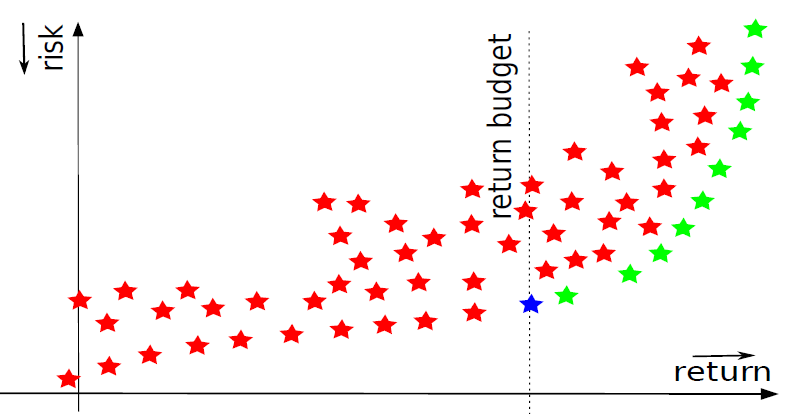
\includegraphics[width=0.35\textwidth]{pics/21sett/budget1.png}\label{subfig:21sett_budget1}}
			\hspace{0.5cm}
			\subfigure[Minimize risk with budget on minimum return,, $\min \{f_{2}(x)~: f_{1}(x) \leq \beta ~:x \in S\}$]{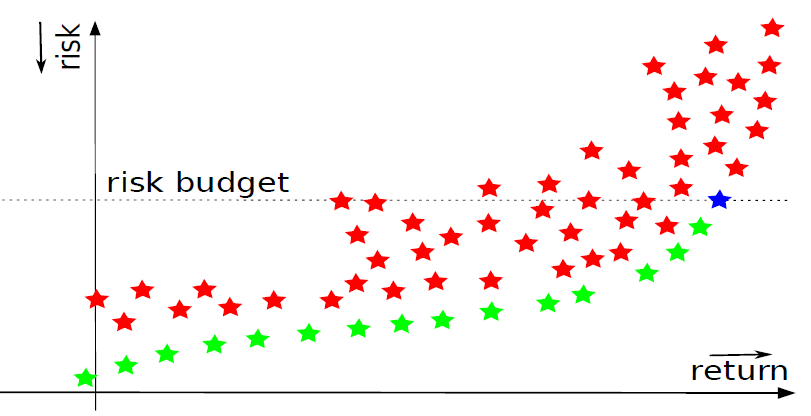
\includegraphics[width=0.35\textwidth]{pics/21sett/budget2.png}\label{subfig:21sett_budget2}}\\
			\caption{Budgeting}
			\label{fig:21sett_budgeting}
		\end{figure}
	
	\end{description}
\end{example}

\section{Infima, suprema and extended reals}
Let us introduce some mathematical background on minimization (maximization).

\begin{definition}[Totally ordered set]
  We say that a set $S$ is \textbf{totally ordered} if $\forall \, x, y \in S$, either $f(x) \leq f(y)$ or $f(y) \leq f(x)$.
\end{definition}

\begin{definition}[Infima and suprema]
  Let $R$ be a totally ordered set and let $s$ be one of its subsets ($S \subseteq R$):
\[
  \underline{s}\text{ is the {\bf infimum} of } S (\underline{s} = \inf S) \text{ iff } \underline{s} \leq s \;\; \forall s \in S  \;\;\wedge\;\;  \forall t > \underline{s} \; \exists \, s \in S \mbox{ s.t. } s \leq t
\]
\[
  \bar{s} \text{ is the {\bf supremum} of } S (\bar{s} = \sup S) \text{ iff } \bar{s} \geq s \;\; \forall s \in S  \;\;\wedge\;\;  \forall t < \bar{s} \; \exists \, s \in S \mbox{ s.t. } s \geq t
\]
\end{definition}

\noindent An attentive reader may notice that it is possible that infima (suprema) do not exist in $\R$.

\begin{definition}[Extended real]
  In the case of unbounded functions the value of infima or suprema are $\infty$, and we call \textbf{extended reals} $\overline{\R} = {-\infty} \cup \R \cup {+\infty}$.
\end{definition}

\begin{property}
	The following holds for the extended reals:
\begin{itemize}
    \item For all $S \subseteq \R, \sup / \inf S \in \overline{\R}$
    \item $\inf S = -\infty $ indicates that there is no (finite) infimum
    \item $\inf \emptyset = \infty$, $\sup \emptyset = -\infty$
\end{itemize}
\end{property}

\section{(Monotone) Sequences in $\R$ and optimization}
\noindent We are interested in studying sequences, because iterative methods start from a certain point and move towards the optimal.


\term{
	We denote a sequence of iterates as $\{ x_i \} \subset S$ and we denote the plugging a function $f$ into such a sequence as $v_i = f ( x_i )$.
}

\begin{definition}[Limit]
  Given a sequence $\{ x_i \}$ the \textbf{limit} for $i \to \infty$ is defined as
\[
  \lim_{i \to \infty} v_i = v ~ \iff ~ \forall \varepsilon > 0 ~ \exists ~ h \text{ s.t. } \abs{v_i - v} \leq \varepsilon ~ \forall i \geq h
\]
\end{definition}

\noindent It may happen that a sequence has or does not have a limit. For example $\{ \frac{1}{n}\}$ has limit $0$ for $n \to +\infty$, while $\{ {(-1)}^n \}$ does not have any.

\begin{proposition}
  Let us be given a monotone sequence, then the sequence \textbf{does} have a limit.
\end{proposition}

Notice that a sequence either is monotone or it can be ``split'' into two monotone sequences.

\begin{example}
	Let us consider the sequence $\{ {(-1)}^n\}$. It does not converge to any value, but it can be split into $\{ {(-1)}^{2n}\}$ and $\{ {(-1)}^{2n+1}\}$ and these two subsequences are both monotone.\\
\end{example}

Forcing monotonicity on sequences in $\R$ can be performed splitting the sequence into a non-decreasing sequence and a non-increasing sequence:
	\[
	\underline{v}_i^* = \inf \{v_h: h\leq i\} \text{ and } \bar{v}_i^* = \sup \{v_h: h\leq i\}
	\]

This way we get $\underline{v}_1 \le \underline{v}_2 \le \ldots$ and $\bar{v}_1 \ge \bar{v}_2 \ge \ldots$ and they have a limit: $\liminf\limits_{i \to \infty} v_i  \lim\limits_{i \to \infty} \underline{v_i}^* = v_\infty^* = f_*$ and  $\limsup\limits_{i \to \infty} v_i  \lim\limits_{i \to \infty} \bar{v}_i^* = v_\infty^* = f_*$

\begin{proposition}
	The following holds:
	\begin{itemize}
		\item $\bar{v}_i \ge \underline{v}_i \Rightarrow \limsup\limits_{i\to \infty} v_i \ge \liminf\limits_{i \to \infty} v_i$
		\item $\lim\limits_{i \to \infty} v_i = v \iff \limsup\limits_{i\to \infty} v_i = v = \liminf\limits_{i \to \infty} v_i$ 
	\end{itemize}	
\end{proposition}

\section{Vector spaces and topology}\label{21sett_sec:vector_space}
For the problems we are going to study, real numbers are used to describe each feature of a dataset and this has the mathematical equivalent in the term ``vector''.

\begin{definition}[Euclidean vector space]
We call \textbf{Euclidean space}
\[
  \R^n :=\biggl \{ \, \begin{pmatrix}x_1\\ x_2\\ \vdots\\ x_n\end{pmatrix}~:~x_i \in \R,~i = 1, \ldots, n \biggr \}
\]
Equivalently, we can characterize the Euclidean space as Cartesian product of $\R$ $n$ times: $\R^n = \R \times \R \times \ldots \R$.
Every vector space and in particular Euclidean spaces are closed under sum and scalar multiplication.
\end{definition}

\noindent The main operations on elements of the Euclidean space (vectors) are:

\begin{description}
  \item[{\sc Sum:}] $\vect{x} + \vect{y} := \begin{pmatrix}x_1 + y_1\\
      x_2 + y_2\\
      \vdots\\
      x_n + y_n\\
  \end{pmatrix}$
\item[{\sc Scalar multiplication:}] $\alpha \vect{x} = \begin{pmatrix}\alpha x_1\\
    \alpha x_2\\
    \vdots\\
    \alpha x_n\\
  \end{pmatrix}$
\end{description}

In linear algebra, $\vect{x} \in \R^n$ is a column vector $\in \R^n$, whenever a row vector is needed for dimensionality issues it is denoted as $\tr{x}$.

\begin{definition}[Basis]
	Any vector $\vect{x} \in \R^n$ can be obtained from a linear combination of a set of vectors that is called ``basis''.
	In Euclidean spaces there exists a special basis that is called ``canonical'', where each vector $\vect{u^i}$ has a $1$ in position $i$ and a $0$ elsewhere.
\end{definition}

\begin{definition}[Finite vector space] Let $V(K, n, m)$ be a vector space. It is said to be \textbf{finite} if its basis have a finite cardinality.
\end{definition}

At this point, it is crucial to observe that not all vector spaces are finite nor they are a totally ordered set.

\noindent In this course we will deal with the concept of limit over a vector space very often and for this purpose we are going to introduce a topology on vector spaces (i.e. norm, scalar product,  distance).

\begin{definition}[Euclidean norm]
 Let $\vect{x} \in \R^n$, we define \textbf{euclidean norm} of $\vect{x}$:
  \[
    \norm{\vect{x}}_2 = \sqrt{\sum\limits_{i=1}^n {x_i}^2} = \sqrt{ \ps{\vect{x}}{\vect{x}}}
  \]
\end{definition}

\begin{proposition}
Any norm on a vector space has the following properties:
\begin{enumerate}
  \item $\norm{\vect{x}} \ge 0$ and $\forall \vect{x} \in \R^n$, $\norm{\vect{x}}=0~\iff~\vect{x}=\vect{0}$;
  \item $\norm{\alpha \vect{x}} = \abs{\alpha} \norm{\vect{x}},~\forall \vect{x} \in \R^n,~\alpha \in \R$;
  \item $\norm{\vect{x}+\vect{y}} \le \norm{\vect{x}} + \norm{\vect{y}},~\forall \vect{x},\vect{y} \in \R^n$ (triangle inequality).
\end{enumerate}
\end{proposition}

\begin{proposition}[Cauchy-Schwartz inequality]
  Let $\vect{x}, \vect{y} \in \R^n$. The following holds:
  \[
    \ps{\vect{x}}{\vect{y}}^2 \;\leq \; \ps{\vect{x}}{\vect{x}}\ps{\vect{y}}{\vect{y}}\equiv \abs{\ps{\vect{x}}{\vect{y}}} \leq \norm{\vect{x}} \norm{\vect{y}},~\forall \vect{x},\vect{y} \in \R^n
  \]
\end{proposition}

\begin{proposition}[Parallelogram Law]
  \[
    2\norm{\vect{x}}^2 + 2\norm{\vect{y}}^2 = \norm{\vect{x} +\vect{y}}^2 + \norm{\vect{x} - \vect{y}}^2
  \]
\end{proposition}

\begin{proposition}
  \[
    \norm{\vect{x}+ \vect{y}}^2 = \norm{\vect{x}}^2 + \norm{\vect{y}}^2 + 2\ps{\vect{x}}{\vect{y}}
  \]
\end{proposition}

The $2$-norm is a special case of the more general $p$-norm.

\begin{definition}[p-norm] Let $p \geq 1$ be a real number, the p-norm of a vector $\vect{x} = ( x_1, \dots , x_n )$ is defined as follow:
  \[
    \norm{\vect{x}}_p := {\left( \sum_{i = 1}^n \abs{x_i}^p\right)}^{1/p}
  \]
We require $p \geq 1$ for the general definition of the $p$-norm because the triangle inequality fails to hold if $p < 1$. 
The $p$-norm is convex for $p \geq 1$ and non convex for $p < 1$.
\end{definition}

The most important $p$-norms are the following:
\begin{itemize}
    \item $\norm{\vect{x}}_1 := \sum_{i = 1}^n \abs{x_i}$
    \item $\norm{\vect{x}}_\infty := \max\{ \abs{x_i}\; :\; i = 1, \dots, n \}$
    \item $\norm{\vect{x}}_i := \abs{\{ i \; : \; \abs{x_i} > 0\}}$
\end{itemize}

\begin{proposition}
For any given finite-dimensional vector space $V(K, n)$ (e.g. $\R^n$), all norms on $V$ are \emph{equivalent} (therefore, convergence in one norm implies convergence in any other norm).
Formally, $ \forall \norm{\cdot}_A\, ,\,\norm{\cdot}_B$:
  \[
    \exists \; 0 < \alpha < \beta \;\; s.t\;\; \alpha\norm{x}_A \leq \norm{x}_B \leq \beta\norm{x}_A \qquad \forall \vect{x} \in V
  \]
\end{proposition}

This rule may not apply in infinite-dimensional vector spaces such as function spaces. For such cases we define the 

\begin{proposition}[Holder's inequality]
  Let $V(K, n)$ be a (possibly infinite) vector space, for any two norms $ \forall \norm{\cdot}_A\, ,\,\norm{\cdot}_B$ the \textbf{Holder's inequality} holds
  \[
    \ps{x}{y}^2 \leq \norm{x}_A \norm{y}_B \; \; 1/A + 1/B = 1
  \]
\end{proposition}

\begin{definition}[Ball]
Let $\vect{\bar{x}} \in \R^n$. We term \textbf{ball} centered in $\bar{\vect{x}}$ and having $\varepsilon$ as radius as the set of points that are close enough to $\vect{x}$: $B(\bar{\vect{x}}, \varepsilon) = \{\vect{x}\in \R^n~:~ \norm{\vect{x} - \bar{\vect{x}}} \le \varepsilon\}$.
\end{definition}

Let us take a unit ball, if the center of the unit-ball is in the origin $(0,0)$, then each point on the unit-ball will have the same $p$-norm (i.e. $1$). The unit ball therefore describes all points that have ``distance'' $1$ from the origin, where ``distance'' is measured by the $p$-norm.
In \Cref{fig:21sett1} we may observe the different shapes of the same ball varying the value of $p$ in the $p$-norm.\\

\addpic{0.4}{pics/21sett/pnorms.pdf}{The shapes of balls centered in the origin of radius $1$ varying the value of $p$-norm.}{fig:21sett1}

\begin{definition}[Standard scalar product]
  Let $\vect{x}, \vect{y} \in \R^n$ we define the \textbf{standard scalar product} between these two vectors as
  \[
\ps{\vect{x}}{\vect{y}} \; := \; \tr{\vect{y}} \vect{x} = \sum_{i=1}^n x_i y_i = x_1 y_1 + \cdots + x_n y_n
  \]
\end{definition}

\begin{proposition}
A scalar product has the following properties:
\begin{enumerate}
  \item $\ps{\vect{x}}{\vect{y}} = \ps{\vect{y}}{\vect{x}} \quad \forall \vect{x}, \vect{y} \in \R^n$ (symmetry)
  \item $\ps{\vect{x}}{\vect{x}} \ge 0,~\forall \vect{x} \in \R^n$, $\ps{\vect{x}}{\vect{x}}=0~\iff~\vect{x}=\vect{0}$;
  \item $\ps{\alpha \vect{x}}{\vect{y}} = \alpha \ps{\vect{x}}{\vect{y}},~\forall \vect{x}\in\R^n, \alpha \in \R$;
  \item $\ps{\vect{x} + \vect{y}}{\vect{z}} = \ps{\vect{x}}{\vect{z}} + \ps{\vect{y}}{\vect{z}},~\forall \vect{x},\vect{y}, \vect{z} \in \R^n$.
\end{enumerate}
\end{proposition}

\noindent An important geometric characterization of the scalar product is the one that uses angles:
\[
  \ps{\vect{x}}{\vect{y}} = \norm{\vect{x}} \norm{\vect{y}} \cos \theta
\]
According to this new definition, we can observe that $\vect{x}$ and $\vect{y}$ are orthogonal ($\vect{x} \perp \vect{y}$) iff $\ps{\vect{x}}{\vect{y}} = 0$ and in all the other cases they somehow point in the same direction.

We could rewrite the scalar product between $\vect{x}$ and $\vect{y}$ as $\tr{\vect{y}} I \vect{x}$, where $I \in D(\R, n)$ is the identity matrix.
Thanks to this observation. we can state the more general form of the scalar product:

\begin{definition}[Scalar product]
Let $\vect{x}, \vect{y} \in `R^n$ and let $M \in M(\R, n)$ be a positive definite matrix (for further details see).
We call \textbf{scalar product} the following 
\[
\ps{\vect{x}}{\vect{y}}_M := \tr{\vect{y}}M\vect{x}
\]
\end{definition}

\todo[inline]{Aggiungere reference al punto in cui si definisce una matrice definita positiva}

\begin{definition}[Euclidean distance]
The \textbf{Euclidean distance} between points $\vect{x}$ and $\vect{y}$ in $\R^n$ is the length of the line segment connecting them.
In Cartesian coordinates, if $\vect{x} = (x_{1}, x_{2}, \ldots, x_{n})$ and $\vect{y} = (y_{1}, y_{2}, \ldots, y_{n})$ are two points in the $n$-dimensional Euclidean space, then the distance ($d$) from $\vect{x}$ to $\vect{y}$, or from $\vect{y}$ to $\vect{x}$ is given by
  \[
    d(\vect{x},\vect{y}) := \lVert \vect{x} - \vect{y} \rVert = \sqrt{{(x_{1} - y_{1})}^{2} + \cdots + {(x_{n} - y_{n})}^{2}} 
  \]
  
\end{definition}
 
 \begin{proposition}
The Euclidean distance has the following properties:
\begin{enumerate}
  \item $d(\vect{x},\vect{y}) \geq 0  \; \forall \vect{x},\vect{y} \in \R^n \; , \; d(\vect{x},\vect{y}) = 0 \iff \vect{x} = \vect{y}$
  \item $d(\alpha \vect{x},0) = \abs{\alpha}d(\vect{x},0) ~ \forall \vect{x} \in \R^n,~ \alpha \in \R$
  \item $ d(\vect{x},\vect{y}) \leq d(\vect{x},\vect{z}) + d(\vect{z}, \vect{y}) ~ \forall \vect{x},\vect{y},\vect{z}  \in \R^n$ (triangle inequality)
\end{enumerate}
\end{proposition}

\section{Limit of a sequence in $\R^n$}
We have now all the tools to define the notion of limit of a sequence in $\R^n$.

\begin{definition}[Limit of a sequence in the Euclidean space]
  Let $\{ \vect{x_i }\} \subset \R^n$ be a sequence in $\R^n$.
  We say that $\{\vect{x_i}\}$ converges to a \textbf{limit} $\vect{x}$ for $i \to +\infty$ and denote $\lim_{i \to \infty} x_i = x$ or $\{ x_i \} \to x$ if $\forall \varepsilon > 0~\exists h~\text{s.t.}~d(\vect{x_i} , \vect{x}) \leq \varepsilon~\forall i \geq h$\\
  or, equivalently, $\forall \varepsilon > 0~\exists h~\text{s.t.}~\vect{x_i} \in \mathcal{B}( \vect{x} , \varepsilon ) \; \forall i \geq h$ \\
  or, even $\lim_{i \to \infty} d( \vect{x_i} , \vect{x} ) = 0$.
\end{definition}

In the definition of limit there is the idea that the points of $\{\vect{x_i}\}$ eventually all come arbitrarily close to $\vect{x}$.
Moreover, since $\R^n$ is not totally ordered, there is no obvious $\liminf$ nor $\limsup$.
\end{document}